\documentclass{standalone}
\usepackage{tikz}
\usepackage{amsmath}
\usetikzlibrary{shapes.geometric, arrows.meta, positioning}

\begin{document}

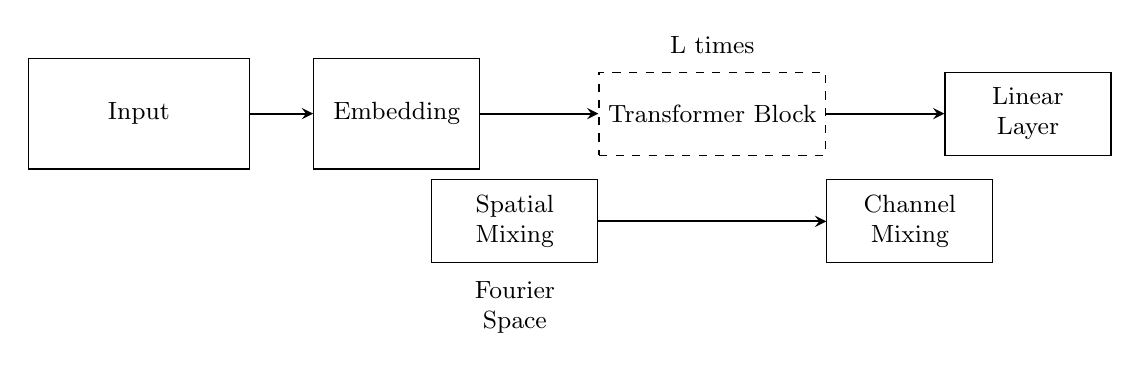
\begin{tikzpicture}[font=\small, node distance=1.5cm, every node/.style={align=center}]

    % Styles
    \tikzstyle{block} = [rectangle, draw, minimum height=3em, minimum width=6em]
    \tikzstyle{arrow} = [thick,->,>=stealth]
    \tikzstyle{dashedblock} = [rectangle, draw, dashed, minimum height=3em, minimum width=5em]

    % Nodes
    \node[block, minimum width=8em, minimum height=4em] (input) {Input};

    \node[block, right=0.8cm of input, minimum height=4em] (embedding) {Embedding};

    \node[dashedblock, right=1.5cm of embedding] (transformerblock) {Transformer Block};
    \node[block, below left=0.3cm and 0cm of transformerblock] (spatial) {Spatial \\ Mixing};
    \node[block, below right=0.3cm and 0cm of transformerblock] (channel) {Channel \\ Mixing};

    \node[block, right=1.5cm of transformerblock] (linear) {Linear \\ Layer};

    % Connections
    \draw[arrow] (input) -- (embedding);
    \draw[arrow] (embedding) -- (transformerblock);
    \draw[arrow] (transformerblock) -- (linear);

    % Dashed box content
    \draw[arrow] (spatial) -- (channel);
    \node[above=0.1cm of transformerblock] {L times};

    % Fourier space label
    \node[below=0.1cm of spatial] {Fourier \\ Space};

\end{tikzpicture}

\end{document}